\chapter{Mercoledì 22/04/2020}
\section{Qualità delle relazioni}
Abbiamo progettato il nostro sistema attraverso un linguaggio concettuale, abbiamo utilizzato il modello E-R, abbiamo verificato le ridondanze e l'efficienza ottenendo alla fine il modello logico, cioè una serie di schemi di relazione. Adesso dobbiamo verificare la \emph{qualità delle relazioni}, cioè se presentano caratteristiche utili per il mantenimento della base di dati.
\paragraph{Obiettivo} Valutare la qualità della progettazione di schemi relazionali, capire se un raggruppamento di attributi in uno schema di relazione sia migliore di un altro.
\paragraph{Approccio adottato} \emph{top-down}.
\paragraph{Obiettivi impliciti}
\begin{itemize}
	\item Conservazione dell'informazione, cioè il mantenimento di tutti i concetti espressi mediante il modello concettuale, inclusi tipi di attributi, tipi di entità e tipi di associazioni.
	\item La minimizzazione delle ridondanze, cioè l'evitare la memorizzazione ripetuta della stessa informazione e quindi la necessità di effettuare molteplici aggiornamenti al fine di mantenere la consistenza tra le diverse copie della medesima informazione.
\end{itemize}
\paragraph{Linee guida}
\begin{itemize}
	\item \textbf{Semplice è bello}! Uno schema di relazione deve essere progettato in modo da rendere semplice la spiegazione del suo significato. Non devo raggruppare attributi provenienti da più tipi di entità e tipi di relazione in un'unica relazione. Se uno schema corrisponde a un solo tipo di entità o a un solo tipo di relazione risulta semplice spiegarne il significato, evitando così l'emergere di ambiguità semantiche.
	\item \textbf{Niente anomalie}! Gli schemi vanno progettati in modo da evitare anomalie nell'inserimento, nella cancellazione o nella modifica. Se possono presentarsi anomalie vanno rilevate e dobbiamo fare in modo che i programmi legati alla base di dati operino in modo corretto.
	\item \textbf{Evitare frequenti valori nulli}! Evitare di porre in una relazione attributi i cui valori possono essere frequentemente nulli. Se questi sono inevitabili ci si assicuri che si presentino solo in casi eccezionali rispetto al numero di tuple di una relazione. 
\end{itemize}
\paragraph{Esempio 1} Prendiamo la seguente relazione
\begin{verbatim}
	Fattura(CodF, CodProd, TotDaPagare, CostoNettoProd, IVA)
\end{verbatim}
Osservo che:
\begin{itemize}
	\item Il codice della fattura (CodF) determina il prodotto comprato, quindi il codice del prodotto (CodProd) e il costo totale (TotDaPagare)
	\item Il codice del prodotto (CodProd) determina il costo netto (CostoNettoProd) e l'iva da pagare (IVA)
	\item CostoNettoProd e IVA determinano quanto bisogna pagare (TotDaPagare)
\end{itemize}
Devo mantenere il tutto consistente. TotDaPagare è determinato da altri attributi, per evitare anomalie conviene rimuoverlo e calcolare il costo totale direttamente nella query.
\paragraph{Esempio 2} Prendiamo la seguente relazione
\begin{verbatim}
	Anagrafe(CF, NomeP, Indirizzo, NomeC, NumAb)
\end{verbatim}
Osservo che :
\begin{itemize}
	\item Il codice fiscale (CF) determina il nome della persona (NomeP), l'indirizzo (Indirizzo) e il nome della città (NomeC)
	\item Il nome della città (NomeC) determina il numero di abitanti (NumAb)
\end{itemize}
Il numero di abitanti è ripetuto tante volte quanti sono i residenti, questo valore deve essere mantenuto consistente (cioè uguale) per ogni persona di una certa città. Risulta ovvio che calcolare per ogni persona il numero di abitanti sia alquanto pesante. \textbf{Come risolviamo?} Trasformiamo Anagrafe in due schemi separati (con vincolo di integrità referenziale su NomeC e un vincolo aggiuntivo su NumAb)
\begin{verbatim}
	Persona(CF, NomeP, Indirizzo, NomeC)
	Residenza(NomeC, NumAb)
\end{verbatim}
\subsection{Approccio formale} 
Abbiamo visto che ci sono attributi che dipendono da altri attributi, devo verificare se ci sono troppe dipendenze tra gruppi di attributi all'interno di una tabella. A tal proposito parliamo di \textbf{dipendenze funzionali}, che esprimono legami semantici tra due gruppi di attributi di uno schema di relazione.
\begin{itemize}
	\item Una dipendenza funzionale è una proprietà dello schema di relazione, non di un particolare stato valido
	\item Una dipendenza funzionale non può essere dedotta a partire da uno stato valido, ma deve essere definita esplicitamente da qualcuno che conosce la semantica degli attributi (quindi non determino proprietà osservando i valori delle istanze, potrei confondere proprietà valide solo per quell'istanza con proprietà dello schema di relazione)
\end{itemize}
\paragraph{Definizione} Consideriamo la relazione $r$ su $R(X)$ e due sottoinsiemi non vuoti $Y$ e $Z$ di $X$. Si dice che esiste in $r$ una dipendenza funzionale da $Y$ a $Z$ se, per ogni coppia di ennuple $t_1$ e $t_2$ di r con gli stessi valori su $Y$ risulta che $t_1$ e $t_2$ hanno gli stessi valori anche su $Z$. \paragraph{Notazione} La notazione adottata è la seguente:
\[Y \longrightarrow Z\]
\paragraph{Attenzione} Non è detto che se io ho $Y \longrightarrow Z$ abbia il contrario, cioè $Z \longrightarrow Y$

\paragraph{Forma normale}
Attraverso le dipendenze funzionali esprimo tutto quello che so riguardante la base di dati. In base a queste dipendenze vorrei costruirmi una caratteristica dello schema per cui valgono quelle dipendenze: ciò significa che se quello schema presenta quelle caratteristiche allora si ha consistenza.\\
Questo schema è detto \textbf{forma normale}, che garantisce l'assenza di particolari difetti dallo schema (determina un livello di qualità). In base alle proprietà che ho dato posso determinare se lo schema si trova in una certa forma normale o in nessuna.
\paragraph{Normalizzazione} Se applico a un certo schema la definizione di forma normale e individuo che questo non è in tale forma, allora compio un processo di \emph{normalizzazione}. La normalizzazione è utilizzata come tecnica di verifica dei risultati della progettazione, non costituisce metodologia di progetto.
\paragraph{Esempio 3} Vediamo la seguente tabella contenente le informazioni di una certa azienda
\begin{center}
	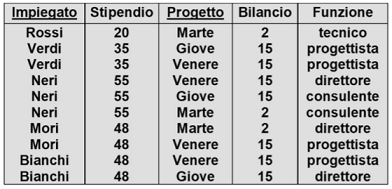
\includegraphics{images/129.PNG}
\end{center}
Abbiamo i cognomi, gli stipendi, i progetti con il loro bilancio e la funzione nel progetto di ciascun dipendente. Ogni impiegato può partecipare a più progetti, sempre con lo stesso stipendio, e con una sola funzione per progetto. Neri, per esempio, lavora su tre progetti differenti.\\
Potrei incorrere nelle seguenti anomalie effettuando modifiche in modo scorretto:
\begin{itemize}
	\item \textbf{Anomalia di aggiornamento}: se lo stipendio di un impiegato varia è necessario andarne a modificare il valore più tuple
	\item \textbf{Anomalia di cancellazione}: se un impiegato si licenzia dobbiamo cancellarlo in diverse tuple (quindi rimuoverlo da tutti i progetti)
	\item \textbf{Anomalia di aggiornamento}: se un progetto varia il suo bilancio devo modificare l'attributo relativo in tutte le tuple dei dipendenti coinvolti nel progetto.
\end{itemize}
La causa sta, ovviamente, nella ripetizione dello stipendio di un impiegato e del bilancio di un progetto. L'errore è stato compiuto proprio nella fase di progettazione: abbiamo usato un'unica relazione per rappresentare gruppi di informazioni eterogenee. Trasformiamo le informazioni dette prima in dipendenze
\begin{itemize}
	\item Ogni impiegato ha un solo stipendio: Impiegato $\longrightarrow$ Stipendio
	\item Ogni progetto ha un solo bilancio: Progetto $\longrightarrow$ Bilancio
	\item Ogni impiegato ha una sola funzione per progetto: Impiegato Progetto $\longrightarrow$ Funzione
\end{itemize}
Osservando la tabella individuiamo pieno rispetto di queste dipendenze. \textbf{Ma ne esistono anche altre?} Abbiamo le cosiddette \textbf{dipendenze banali}, che sono sempre soddisfatte (proprietà ovvie di una relazione). Si osserva 
\[Impiegato\;Progetto \longrightarrow Progetto\]
Si dice che:
\begin{itemize}
	\item $Y \to A$ è non banale se $A$ non compare tra gli attributi di $Y$
	\item $Y \to Z$ è non banale se nessun attributo in $Z$ appartiene a $Y$.
\end{itemize}
\paragraph{Legame tra dipendenze e anomalie} Osserviamo che le prime due dipendenze comportano ripetizioni, mentre la terza no. Impiegato e Progetto non sono chiavi, Impiegato Progetto è chiave! La relazione contiene alcune informazioni legate alla chiave e altre ad attributi che non lo sono.

\subsection{Teoria delle dipendenze}
\subsubsection{Implicazione}
Sia $F$ un insieme di dipendenze funzionali definite su $R(Z)$ e sia $X \longrightarrow Y$.
\begin{itemize}
	\item Si dice che $F$ implica la dipendenza $X \to Y$ ($F \Rightarrow X \to Y$) se per ogni istanza $r$ di $R$ che verifica tutte le dipendenze in $F$, risulta verificata anche $X \to Y$.
	\item Si dice anche che $X \to Y$ è implicata da $F$
\end{itemize}
\subsubsection{Chiusura}
Dato un insieme di dipendenze funzionali $F$ definite su $R(Z)$ la chiusura di $F$ è l'insieme di tutte le dipendenze funzionali implicate da $F$.
\[F^{+}=\{X \to Y | F \Rightarrow X \to Y\}\]
Dato un insieme di dipendenze funzionali $F$ definite su $R(Z)$, un'istanza $r$ di $R$ che soddisfa $F$ soddisfa anche $F^{+}$.
\subsubsection{Superchiave}
Dato $R(Z)$ ed un insieme $F$ di dipendenze funzionali, un insieme di attributi $K$ appartenenti a $Z$ si dice superchiave di $R$ se la dipendenza funzionale $K \to Z$ è logicamente implicata da $F$ ($K\to Z$ è in $F^{+}$)
\paragraph{Chiave} Se nessun sottoinsieme proprio di $K$ è superchiave di $R$ allora $K$ si dice chiave di $R$.
\subsection{Calcolo di $F^{+}$ (regole di Armstrong)}
Utilizziamo un approccio costruttivo per arrivare all'algoritmo. Esistono una serie di regole, definite da \emph{Armstrong}, che mi permettono di arrivare a trovare l'insieme di tutte le dipendenze funzionali presenti nella chiusura.
\paragraph{Regole di inferenza di Armstrong}
\begin{itemize}
	\item \textbf{Riflessività}: se $Y \subseteq X$, allora $X \to Y$
	\item \textbf{Additività (o espansione)}: se $X \to Y$, allora $XZ \to YZ$ per qualunque $Z$
	\item \textbf{Transitività}: se $X \to Y$ e $Y \to Z$ allora $X \to Z$
\end{itemize}
\paragraph{Regole derivate di Armstrong}
\begin{itemize}
	\item \textbf{Regola di unione}: $\{X\to Y, X \to Z\} \Rightarrow X \to YZ$
	\item \textbf{Regole di pseudotransitività (o aggiunta sinistra)}: $\{X\to Y, WY \to Z\} \Rightarrow XW \to Z$
	\item \textbf{Regola di decomposizione}: se $Z \subseteq Y, X \to Y \Rightarrow X \to Z$
\end{itemize}
\paragraph{Proprietà delle regole di Armstrong}
\begin{itemize}
	\item \textbf{Teorema correttezza}: le regole di inferenze sono corrette, cioè, applicandole a un insieme F di dipendenze funzionali, si ottengono solo dipendenze logicamente implicate da F.
	\item \textbf{Teorema completezza}: le regole di inferenza sono complete, cioè, applicandole ad un insieme F di dipendenze funzionali, si ottengono tutte le dipendenze logicamente implicate da F.
	\item \textbf{Teorema minimalità}: le regole di inferenza sono minimali, cioè, ignorando anche una sola di esse, l'insieme di regole che rimangono non è più completo.
\end{itemize}
\paragraph{Esempio di dimostrazione} Dimostrare che per ogni istanza di relazione
\[X \to Y \Rightarrow XZ \to YZ\]
Supponiamo per assurdo che esista un'istanza $r$ di $R$ in cui valga $X \to Y$ ma non $XZ \to YZ$. Devono esistere due tuple $t_1$ e $t_2$ di $r$ tali che:
\begin{enumerate}
	\item $t_1[X]=t_2[X]$
	\item $t_1[Y] = t_2[Y]$
	\item $t_1[XZ]=t_2[XZ]$
	\item $t_1[YZ]\neq t_2[YZ]$
\end{enumerate}
Cioè è assurdo. Dalla prima e dalla terza deduciamo che
\[t_1[Z] = t_2[Z]\]
con questa e la seconda concludiamo che
\[t_1[YZ]=t_2[YZ]\]
in contraddizione con la quarta!

\paragraph{Riprendiamo l'esempio 3} Avevamo le seguenti dipendenze funzionali:
\begin{itemize}
	\item Impiegato $\longrightarrow$ Stipendio
	\item Progetto $\longrightarrow$ Bilancio
	\item Impiegato Progetto $\longrightarrow$ Funzione
\end{itemize}
Utilizzando la \emph{regola di attività} sulle prime due otteniamo
\begin{itemize}
	\item Impiegato Progetto $\longrightarrow$ Stipendio Progetto
	\item Impiegato Progetto $\longrightarrow$ Bilancio Impiegato
	\item Impiegato Progetto $\longrightarrow$ Funzione (Uguale a prima)
\end{itemize}
Infine, con la \emph{regola di unione}, avremo
\begin{itemize}
	\item Impiegato Progetto $\longrightarrow$ Stipendio Progetto Impiegato Bilancio Funzione
\end{itemize}
Quindi \underline{Impiegato Progetto} è chiave. Posso trovare altre dipendenze funzionali in $F^{+}$?
\subsection{Equivalenza}
Dato un insieme $F$ di dipendenze funzionali è molto utile poter determinare se un insieme $G$ sia equivalente ad $F$. Affermo che $F$ e $G$ sono equivalenti se
\[F^{+}=G^{+}\]
cioè per ogni $X \to Y \in F$ deve essere \[X \to Y \in G^{+}\] e, viceversa, per ogni $X \to Y \in G$ deve essere \[X \to Y \in F^{+}\]
\paragraph{Esempio} Supponiamo di avere questi due insiemi
\begin{align*}
	F&=\{\ A \to C, AC \to D, E \to AD, E \to H \}\\
	G&=\{\ A \to CD, E \to AH \}
\end{align*}
Voglio verificare l'equivalenza di $F$ e $G$. Devo dimostrare che le dipendenze funzionali in $F$ sono derivabili dalle dipendenze funzionali in G, e viceversa.
\begin{itemize}
	\item $A \to CD \Rightarrow \boxed{A \to C}, A \to D$
	\item $A \to CD, CCD \to CD \Rightarrow AC \to CD \Rightarrow AC \to C, \boxed{AC \to D}$
	\item $E \to AH \Rightarrow E \to A, \boxed{E \to H}$
	\item $E \to A, A \to D \Rightarrow E \to D$
	\item $E \to A , E \to D \Rightarrow \boxed{E \to AD}$
\end{itemize}
Ovviamente dovremo fare la stessa cosa al contrario. Da tutto questo capiamo quanto sia costoso il calcolo di $F^{+}$. Generalmente ci interessa sapere se $F^{+}$ contiene una certa dipendenza.
\paragraph{Chiusura transitiva} Come alternativa posso utilizzare la \emph{chiusura transitiva} di un insieme di attributi $X$ rispetto a $F$. Data una relazione $R(U)$, un insieme di attributi $X \subseteq U$, la chiusura detta consiste nell'insieme degli attributi che dipendono da $X$ (esplicitamente o implicitamente).
\[X^{+F}=\{A \;|\; A \in U\;\land\;F\Longrightarrow X \to A\}\]
Posso dimostrare che $X \to Y$ è in $F^{+}$ se $Y \subseteq X^{+}$
\paragraph{Riprendiamo l'esempio} Invece di verificare se $X \to Y$ in $F$ è anche in $G^{+}$ verifico se $Y \subseteq (X)^{+G}$ (chiusura di $X$ rispetto a $G$). Le varie chiusure qua sotto sono state trovate analizzando l'insieme di dipendenze funzionali $G$.
\begin{itemize}
	\item per $A \to C$ risulta $(A)^{+G}=ACD$. Ok ho $C \subseteq (A)^{+G}$
	\item per $AC \to D$ risulta $(AC)^{+G}=ACD$. Ok ho $D \subseteq (AC)^{+G}$
	\item per $E \to AD$ risulta $(E)^{+G}=EADCH$. Ok ho $AD \subseteq (E)^{+G}$
	\item per $E \to H$ risulta $(E)^{+G}=EHADC$. Ok ho $H \subseteq (E)^{+G}$
\end{itemize}
E viceversa per ogni dipendenza funzionale in G.

\paragraph{Esempio 2} Supponiamo di avere il seguente insieme
\[F = \{  A \to B, BC \to D, B \to E, E \to C \}\]
Calcoliamo $A^{+}$, cioè l'insieme di attributi dipendenti da $A$. Trovo che
\begin{itemize}
	\item $A^{+} = A$
	\item $A^{+} = AB$ poichè $A \to B$ e $A \subseteq A^{+}$
	\item $A^{+} = ABE$ poichè $B \to E$ e $B \subseteq A^{+}$
	\item $A^{+} = ABEC$ poichè $E \to C$ e $E \subseteq A^{+}$
	\item $A^{+} = ABECD$ poichè $BC \to D$ e $BC \subseteq A^{+}$
\end{itemize}
Quindi da $A$ dipendono tutti gli attributi dello schema, ovvero $A$ è superchiave oltre che chiave.
\subsection{Definizione aggiornata di equivalenza} Abbiamo modificato la definizione di equivalenza. Dati $F$ e $G$, essi sono equivalenti se
\begin{itemize}
	\item per ogni $X \to Y \in F, Y \in X^{+G}$, e
	\item per ogni $Z \to W \in G, W \in Z^{+F}$.
\end{itemize}
\subsection{Importanza della chiusura in un insieme di attributi} Dato $R(Z)$ con le sue dipendenze $F$, la chiusura di un insieme $X \subseteq Z$ di attributi è fondamentale per diversi scopi:
\begin{itemize}
	\item Possiamo verificare se una dipendenza funzionale è logicamente implicata da $F$
	\[X \to Y \in F^+ \Longleftrightarrow Y \subseteq X^{+F}\]
	\item Possiamo verificare se un insieme di attributi è chiave o superchiave:
	\begin{itemize}
		\item $X$ è superchiave di $R$ se e solo se $X \to Z \in F^+$, cioè se e solo se $Z \subseteq X^{+F}$
		\item $X$ è chiave di $R$ se e solo se $X \to Z \in F^+$ e non esiste alcun sottoinsieme $Y \subset X$ eliminando almeno un elemento, tale che $Z \subseteq Y^{+F}$
	\end{itemize}
\end{itemize}
\subsection{Ridondanze di un insieme di dipendenze funzionali}
Alcuni attributi di una dipendenza funzionale possono essere ridondanti. L'obiettivo è individuare forme equivalenti più semplici! Posso semplificare rimuovendo attributi sul lato sinistro di una DF (poichè non essenziali per determinare la parte destra) o rimuovere intere DF poichè ridondanti. Ricorriamo alle regole di Armstrong:
\begin{itemize}
	\item Applicazione della \emph{Regola di unione}: $\{A \to B, B \to C, A \to CD \}$ può essere semplificata in  $\{A \to B, B \to C, A \to C, A \to D \}$
	\item Attributi estranei a sx:  $\{A \to B, B \to C, AC \to D \}$ può essere semplificata in  $\{A \to B, B \to C, A \to D \}$
\end{itemize}
Un insieme $F$ di dipendenze funzionali può contenere dipendenze ridondanti, ovvero ottenibili tramite altre dipendenze di $F$. Ricorriamo alla transitività: $A \to C$ è ridondante in $\{A \to B, B \to C, \boxed{A \to C}\}$. Ricordiamo che la regola fondamentale è semplificare al massimo la rappresentazione dell'informazione.
\subsection{Dipendenze funzionali semplici}
Possiamo portare un insieme di dipendenze funzionali $F$ in forma standard, quella in cui sulla destra c'è un solo attributo.\\
Il seguente insieme 
\[F=\{AB \to CD, AC \to DE\}\]
Possiamo riscriverlo così
\[F=\{AB \to C, AB \to D, AC \to D, AC \to E\}\]
Quanto fatto è solo un primo step.
\subsection{Attributi estranei}
In alcune dipendenze funzionali è possibile che ci siano attributi inutili (appunto estranei) sul lato sinistro. Come li identifico?
\begin{itemize}
	\item Supponiamo di avere $F = \{AB \to C, A \to B\}$ 
	\item Ho $A^+=A$ e $B^+=B$
	\item $A^+=AB$ poichè $A \to B$ e $A \subseteq A^+$
	\item $A^+=ABC$ poichè $AB \to C$ e $AB \subseteq A^+$
\end{itemize}
$C$ dipende solo da $A$, e in $AB \to C$ l'attributo $B$ è estraneo poichè a sua volta dipende da $A$. Possiamo riscrivere l'insieme di dipendenze funzionali nel seguente modo
\[F^+ = \{ A \to C, A \to B\}\]
\paragraph{Morale della favola} In una dipendenza funzionale del tipo $AX \to B$ l'attributo $A$ è estraneo se $X^+$ include $B$ (ovvero $X$ da solo determina $B$).
\subsection{Algoritmo per la ridondanza di una dipendenza funzionale}
Dopo aver eliminato gli attributi estranei si deve verificare se sono presenti intere dipendenze funzionali inutili, cioè se intere dipendenze funzionali sono implicate da altre. Come faccio a capire se una dipendenza del tipo $X \to A$ è ridondante?
\begin{itemize}
	\item La elimino dall'insieme $F$
	\item Calcolo la chiusura di $X$ ($X^+$)
	\item Verifico se include $A$, cioè se con le dipendenze funzionali che restano riusciamo ancora a dimostrare che $X \to A$
\end{itemize}
\subsection{Copertura minimale}
Un insieme di dipendenze funzionali $F$ è minimale se:
\begin{itemize}
	\item Nella parte destra di ogni dipendenza funzionale c'è un solo attributo
	\item Non si possono togliere attributi nella parte sinistra di qualche FD senza perdere l'equivalenza nell'insieme ottenuto con $F$
	\item Non si possono togliere intere dipendenze funzionali senza perdere l'equivalenza nell'insieme ottenuto con $F$
\end{itemize}
Segue che una copertura minimale di un insieme $F$ è un insieme equivalente a $F$, ma di complessità minore.
\paragraph{NB} La copertura minimale non è unica.
\paragraph{Esempio di individuazione di copertura minimale} 
\begin{itemize}
	\item Abbiamo il seguente insieme: $F=\{ AB \to C, B \to A, C \to A \}$
	\item $A$ è estraneo in $AB \to C$, quindi: $F=\{ B \to C, B \to A, C \to A \}$
	\item $B\to A$ è ridondante, quindi ottengo: $F=\{ B \to C, C \to A \}$
\end{itemize}
Osserviamo che la dipendenze funzionale ridondante non può essere eliminata se prima non eliminiamo l'attributo estraneo. Segue l'importanza dello svolgere i passi spiegati nell'ordine mostrato!